\section{Définitions et propriétés des principaux quadrilatères particuliers}

\begin{definition}
Le \MotDefinition{parallélogramme}{} :

Un quadrilatère dont les côtés opposés sont \textcolor{C2}{\textbf{parallèles deux à deux}} est un parallélogramme. \\[-5em]
\begin{minipage}[t]{0.76\linewidth}
\textcolor{H1}{\textbf{Propriétés}} : dans un parallélogramme :
\begin{itemize}
 \item Les côtés opposés sont \textcolor{H1}{\textbf{parallèles}} et ont \textcolor{H1}{\textbf{la même longueur}} ;
 \item Les diagonales se coupent \textcolor{H1}{\textbf{en leur milieu}} ;
 \item Les angles opposés sont \textcolor{H1}{\textbf{égaux}}.
 \end{itemize}
 \end{minipage}
 \begin{minipage}[c]{0.18\linewidth}
 \vspace{1cm}
  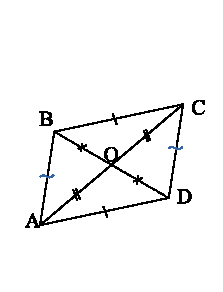
\includegraphics[width=2.5cm]{losangeABCDO}
  \end{minipage} \\
\end{definition}

\begin{minipage}[t]{0.49\linewidth}
\begin{center} 
\includegraphics[width=0.8cm]{flash_droite} \end{center}
 \end{minipage}
 \begin{minipage}[t]{0.49\linewidth}
\begin{center} 
\includegraphics[width=1.1cm]{flash_gauche} \end{center}
 \end{minipage} \\[-2em]

\begin{minipage}[t]{0.49\linewidth}
  \begin{definition}
   Le \MotDefinition{rectangle}{} :
   Un quadrilatère qui a \textcolor{C2}{\textbf{4 angles droits}} est un rectangle.
   
    \begin{center}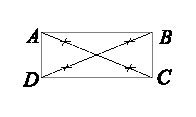
\includegraphics[width=3.5cm]{rectangleABCD}\end{center}
    
   \textcolor{H1}{\textbf{Propriétés}} :
    \begin{itemize}
     \item Un rectangle est un \textcolor{H1}{\textbf{parallélogramme}} donc il possède toutes les propriétés d'un \textcolor{H1}{\textbf{parallélogramme}} ;
     \item Les diagonales d'un rectangle ont \textcolor{H1}{\textbf{la même longueur}}.
     \end{itemize}
   \end{definition}
 \end{minipage}
 %
 \begin{minipage}[t]{0.59\linewidth}
   \begin{definition}
   Le \MotDefinition{losange}{} :
   Un quadrilatère qui a \textcolor{C2}{\textbf{4 côtés de même longueur}} est un losange.
   
     \begin{center}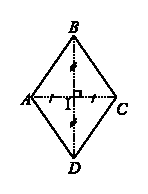
\includegraphics[width=2cm]{losangeABCD2}\end{center}
    
   \textcolor{H1}{\textbf{Propriétés}} :
    \begin{itemize}
     \item Un losange est un \textcolor{H1}{\textbf{parallélogramme}} donc il possède toutes les propriétés d'un \textcolor{H1}{\textbf{parallélogramme}} ;
     \item Les diagonales d'un losange se coupent \textcolor{H1}{\textbf{en leur milieu}} et sont \textcolor{H1}{\textbf{perpendiculaires}}.
     \end{itemize}
   \end{definition}
  \end{minipage} \\
  
\begin{minipage}[t]{0.49\linewidth}
\begin{center} 
\includegraphics[width=1.1cm]{flash_gauche} \end{center}
 \end{minipage}
 \begin{minipage}[t]{0.49\linewidth}
\begin{center} 
\includegraphics[width=0.8cm]{flash_droite} \end{center}
 \end{minipage} \\ [-2em]
  
\begin{definition}
Le \MotDefinition{carré}{} :

Un quadrilatère qui a \textcolor{C2}{\textbf{4 côtés de même longueur et 4 angles droits}} est un carré. \\[-3em]
\begin{minipage}[t]{0.7\linewidth}
\textcolor{H1}{\textbf{Propriétés}} :
\begin{itemize}
 \item Un carré est à la fois \textcolor{H1}{\textbf{un parallélogramme}}, \textcolor{H1}{\textbf{un losange}} et \textcolor{H1}{\textbf{un rectangle}} donc il a toutes les propriétés de ces quadrilatères ;
 \item Les diagonales d'un carré sont \textcolor{H1}{\textbf{perpendiculaires}} et \textcolor{H1}{\textbf{de même longueur}}.
 \end{itemize}
 \end{minipage}
 \begin{minipage}[c]{0.18\linewidth}
 \vspace{1cm}
 \centering
  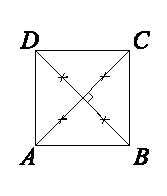
\includegraphics[width=2cm]{carreABCD}
  \end{minipage} \\
\end{definition}



\section{Méthodes de construction}

\begin{methode*1}[Construire un parallélogramme avec la règle et l'équerre]

\vspace{0.8em}
\textcolor{H1}{\textbf{Remarque}} : On utilise ici le fait que les côtés opposés sont parallèles deux à deux.

\begin{exemple*1}
Soient trois points $A$, $B$ et $C$ non alignés. Place le point $D$ tel que $ABCD$ soit un parallélogramme.\\[0.5em]


\begin{tabularx}{\textwidth}{X|X|X}
 \qquad 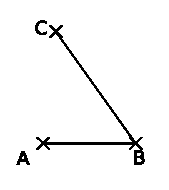
\includegraphics[width=2.1cm]{angleABC8} & 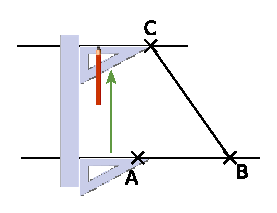
\includegraphics[width=3cm]{angle_parallele} & 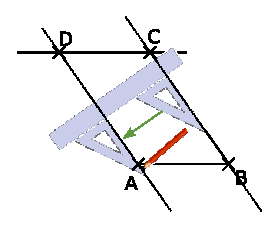
\includegraphics[width=3cm]{quadABCD} \\ 
 On trace les côtés $[AB]$ et $[BC]$ du quadrilatère $ABCD$. Le quadrilatère $ABCD$ est un parallélogramme, donc ses côtés opposés sont parallèles deux à deux : soit $(AB) \parallel (CD)$. & On trace la parallèle à $(AB)$ passant par $C$. & On trace la parallèle à $(BC)$ passant par $A$. Ces deux droites sont sécantes en $D$.
 
 Ainsi $ABCD$ a ses côtés opposés parallèles deux à deux, c'est donc bien un parallélogramme. \\
\end{tabularx} \\[1em]

\end{exemple*1}

\exercice
Réalise un croquis avant de construire le parallélogramme $PRLG$ tel que $PR = 5$ cm, $PG = 6$ cm et  $\widehat{RPG} = 74^\circ$ en utilisant la propriété sur le parallélisme des côtés opposés du parallélogramme.
%\correction

\end{methode*1}

\newpage





\begin{methode*1}[Construire un parallélogramme avec le compas]

 
\vspace{0.8em}
\textcolor{H1}{\textbf{Remarque}} : On utilise ici le fait que les côtés opposés d'un parallélogramme sont égaux deux à deux.

 \begin{exemple*1}
 
  \begin{tabularx}{\textwidth}{X|X|X}
 \qquad 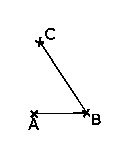
\includegraphics[width=1.2cm]{angleABC_2} & \qquad 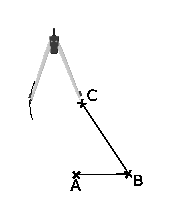
\includegraphics[width=1.9cm]{compasABC} & 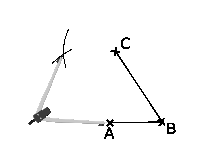
\includegraphics[width=2.4cm]{compasABCD}  \\ 
 On trace les côtés $[AB]$ et $[BC]$ du quadrilatère $ABCD$.
 
 Le quadrilatère $ABCD$ est un parallélogramme, donc ses côtés opposés $[AB]$ et $[CD]$ sont de la même longueur deux à deux : soit $AB = CD$ et $BC = AD$. & À l'aide du compas, on reporte la longueur $AB$ à partir du point $C$. & On reporte la longueur $BC$ à partir du point $A$. On place le point $D$ à l'intersection des deux arcs de cercle puis on trace les côtés $[AD]$ et $[CD]$.
 
Ainsi $ABCD$ a ses côtés opposés égaux deux à deux, c'est donc bien un parallélogramme.\\
\end{tabularx} \\
 
 \end{exemple*1}

\vspace*{1em}
Pour les deux exemples ci-dessous, faire un croquis avant de faire le tracé précis :\\[-2.5em]

\exercice
Construis le parallélogramme $DRAP$ tel que $DR = 6$ cm, $DP = 8$ cm et $\widehat{RDP} = 40^\circ$ en utilisant la propriété sur l'égalité des longueurs des côtés opposés du parallélogramme.
%\correction

\vspace{2.7cm}

\exercice
Construis un rectangle $ABCD$ tel que $AB = 3$ cm et $BC = 5$ cm.
%\correction

\end{methode*1}

%%%%%%%%%%%%%%%%%%%%%%%%%%%%%%%%%%%%%%%%%%%%%%%%%%%%%%%%%%%%

\begin{methode*1}[Construire un losange avec le compas]
 
\vspace{0.8em}
\textcolor{H1}{\textbf{Remarque}} : On utilise ici le fait qu'un losange a quatre côtés de même longueur.

\begin{exemple*1}
Construis un losange $ABCD$ de 6 cm de côté.\\[1em]
\begin{minipage}[c]{0.7\linewidth}
On fait d'abord un croquis. Dans un losange, les quatre côtés ont la même longueur. Ainsi, les triangles $ABD$ et $CBD$ sont \textbf{isocèles} respectivement en $A$ et $C$.
 \end{minipage} \hfill%
 \begin{minipage}[c]{0.24\linewidth}
  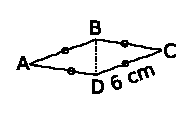
\includegraphics[width=2.6cm]{losange_croquis}
  \end{minipage} \\
  
\begin{tabularx}{\textwidth}{X|X}
 \qquad 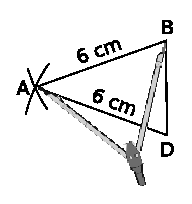
\includegraphics[width=2.6cm]{triangleABD} & 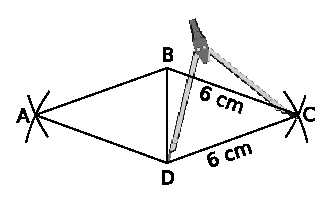
\includegraphics[width=4.8cm]{losangeABCD} \\ 
 On trace un segment $[BD]$. On construit un triangle $ABD$ isocèle en $A$ tel que $AB = AD = 6$ cm. & On construit le triangle $CBD$ isocèle en $C$ tel que $CB = CD = 6$ cm. \\
\end{tabularx} \\

 \end{exemple*1}

\exercice
Construis un losange $VERT$ tel que $VE = 4,5$ cm et $ET = 6,9$ cm.
%\correction

\vspace{3.5cm}

\exercice
Construis un triangle $BOL$ isocèle en $B$ tel que $BO = 2,1$ cm et $OL = 3,4$ cm. Place le point $S$ pour que $BOSL$ soit un losange.
%\correction

\end{methode*1}

%%%%%%%%%%%%%%%%%%%%%%%%%%%%%%%%%%%%%%%%%%%%%%%%%%%%%%%%%%%%

